\documentclass{article}
\usepackage[utf8]{inputenc}
\usepackage{graphicx}
\usepackage{titlepic}
\usepackage{caption}
\usepackage{subcaption}
% \documentclass{beamer}

\newcommand{\namesigdate}[2][5cm]{%
  \begin{tabular}{@{}p{#1}@{}}
    #2 \\[0.4\normalbaselineskip] \hrule \\[0pt]
    {\small } \\[2\normalbaselineskip] 
  \end{tabular}
}

\title{\vspace*{\fill} \textbf{Video Description using Deep Learning}
	  \\ {\large \textbf{Summer Undergraduate Research Award}}
	  \\  \vspace{3mm} 
\includegraphics[width=5cm]{logo.png}}

\author{
	\textbf{Suyash Agrawal}\\ 
	2015CS10262\\
	Computer Science\\
	CGPA: 9.92 \\
	Mob: 9717060183\\
	cs1150262@iitd.ac.in
	\and
	\textbf{Madhur Singhal}\\ 
	2015CS10235\\
	Computer Science\\
	CGPA: 8.66\\
	Mob: 9540972599\\
	cs1150235@iitd.ac.in
}
\date{\textbf{Supervisor:-} \\ \textbf{Subhashis Banerjee} \\ Professor \\ Department of CSE \\ suban@cse.iitd.ac.in\\ IIT Delhi\\
\vspace*{\fill}}




\begin{document}
		% 
\includegraphics{logo.png}
	\maketitle

% \noindent \namesigdate{} \hfill \namesigdate[3cm]{Saroj Kaushik \\ HOD CSE }
% \begin{flushleft}
% \noindent \namesigdate{} 
% \end{flushleft}

\begin{center}
\noindent\rule{3.2cm}{0.4pt} 
\end{center}

\begin{flushright}
\noindent\rule{3.2cm}{0.4pt} 
\\ \textbf{Prof. S. Arun Kumar}
\\ Head of Department
\\ Department of CSE
\\ sak@cse.iitd.ernet.in
\end{flushright}


	\newpage
	% \begin{figure}
% \end{figure}
	
	\section{Introduction}
		\textit{\textbf{Video Description}} is the process of discovering knowledge, structures, patterns and events of interest in the video data and describing them in natural language. Video Description is an incredibly hard problem in computer vision and currently the only source of video description is manual labour. 
		\newline
		Video Description has wide variety of applications. It can help visually impared people "see" the world by describing the scene around them. It has also use in automated survelliance by analysing the videos in real time and reporting criminal activites. Also, it can be used to efficiently index large video databases based upon their content for ease of accessibility.

		\begin{figure}[ht!]
		\centering
		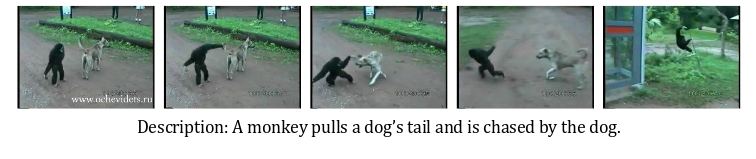
\includegraphics[width=12.5cm]{description.png}
		\caption{Sample Video Description\label{fig0}}
		\end{figure}		
		
%		\begin{figure}[ht!]
%			\centering
%			\begin{subfigure}{.5\textwidth}
%			  	\centering
%			  	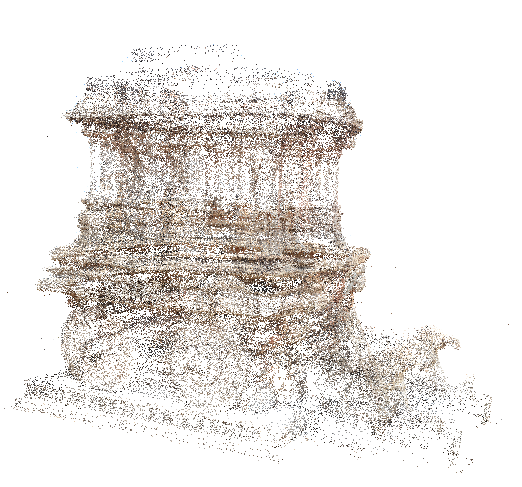
\includegraphics[width=1.0\linewidth]{sparse_chariot.png}
%			  	\caption{Sparse reconstruction}
%			  	\label{fig:sub1}
%			\end{subfigure}%
%			\begin{subfigure}{.5\textwidth}
%			  	\centering
%			  	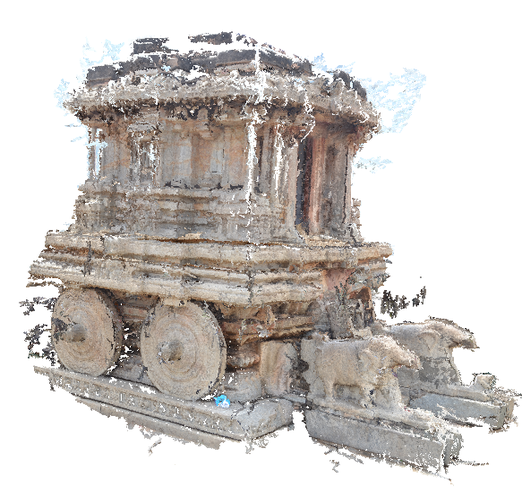
\includegraphics[width=1.0\linewidth]{dense_chariot.png}
%			  	\caption{Dense reconstruction}
%			  	\label{fig:sub2}
%			\end{subfigure}
%			\caption{3D reconstruction}
%			\label{figstart}
%		\end{figure}


		Figure~\ref{fig0} shows a possible description of a sample video.\newline

%		The proposed \textit{pipeline} for this project is shown in Figure~\ref{fig3}.
%
%		\begin{figure}[ht!]
%		\centering
%		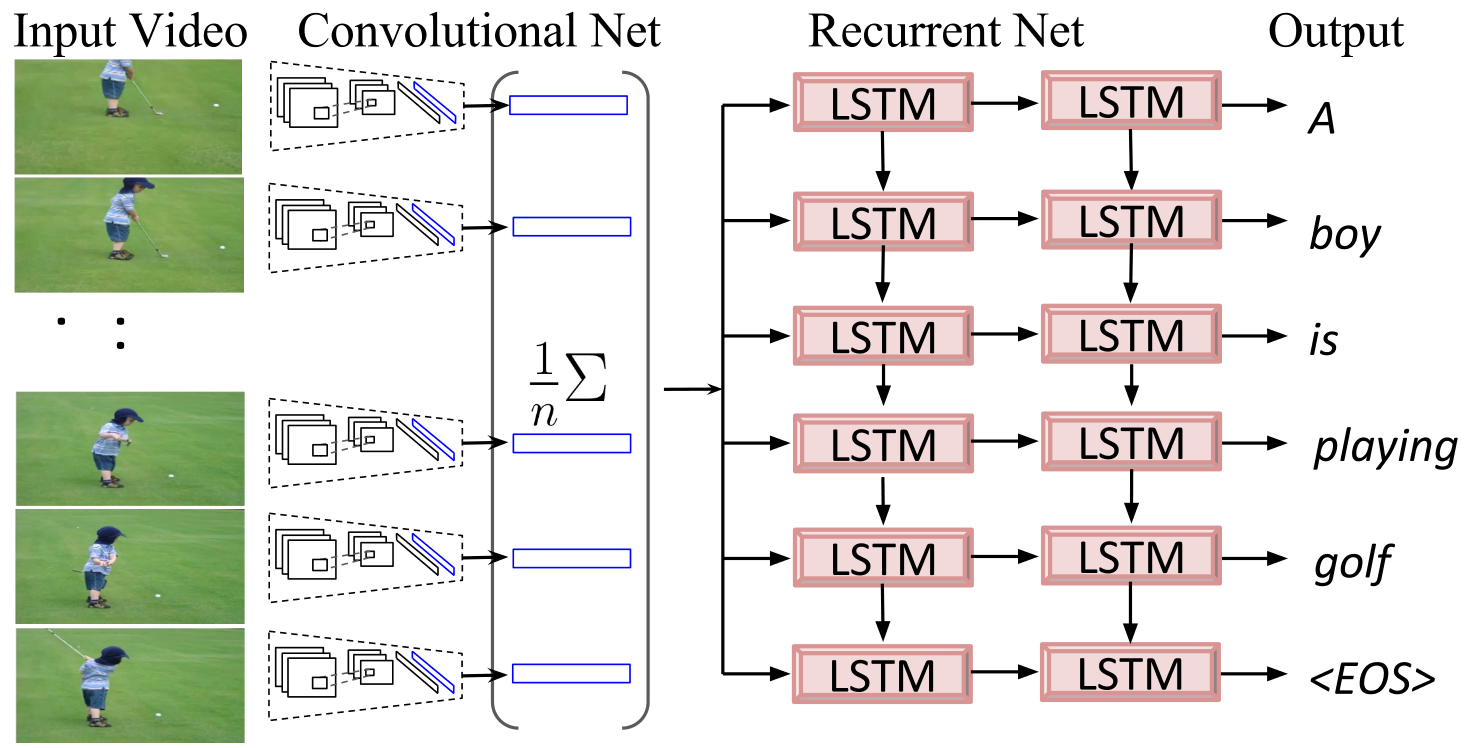
\includegraphics[width=13cm]{pipeline.png}
%		\caption{Proposed pipeline\label{fig3}}
%		\end{figure}
		Most prior work has been done on generating natural language descriptions from images. Past two years have seen a lot of breakthroughs in image captioning problem but so far this has not been used for generating descriptions from videos.\newline
		Our aim is to use these new techniques of image captioning and use them to generate natural language descriptions from video data. In short, we will first encode video data using CNNs and then use RNNs to generate descriptions of these videos. Further, we will also explore using attention models to improve description of videos.

%
%		The processing parts are:
%			\begin{itemize}
%			\item \textit{Intrinsic and extrinsic parameters}: The camera projection matrix is a $3 \times 4$ matrix which represents the pinhole geometry of a camera for mapping 3D points in the world coordinates to 2D points on images. This matrix depends on extrinsic and intrinsic parameters. The intrinsic parameters mainly comprises of focal length, image sensor format, and principal points. The extrinsic parameters define the position of the camera center and the camera's heading in world coordinates in terms of a rigid rotation and translation. 
%			\item \textit{Stereo correspondence generation}: Given two or more images of the same 3D scene, taken from different points of view, the correspondence problem refers to the task of finding a set of points in one image which can be identified as the same points in another image. To do this, points or features in one image are matched with the corresponding points or features in another image. The images can be taken from a different point of view, at different times, or with objects in the scene in general motion relative to the camera(s).
%			\item \textit{Triangulation}: Triangulation refers to the process of determining a point in 3D space given, its projections onto two or more images and their corresponding camera projection matrices. This point is found as the intersection of the two or more projection rays formed from the inverse projection of the 2D image points representing that 3D point in space.
%			\item \textit{Initial point cloud and 3D sparse reconstruction}: As the word suggests, \textit{3D sparse construction} is done for only some set of data points in the given coordinate system called \textit{initial point cloud}. Figure~\ref{fig:sub1} illustrates a 3D sparse construction of a chariot. Figure~\ref{fig:sub2} illustrates 3D dense construction of the same initial point cloud.
%
%			\end{itemize}
	\section{Objectives}
		Our main objective is to understand videos and generate natural language descriptions of them. This task can be further subdivided into following subtasks:
		\begin{enumerate}
			\item
				To ready all available datasets and organize them into training, validation and testing sets.
			\item
				To construct CNNs with pretrained weights for image captioning.
			\item
				To construct Long Short Term Memory (LSTM) Encoder Decoders.
			\item
				To train the network using the test set data and use validation set data for setting hyper-parameters.
			\item
				To benchmark results and improve using techniques like attention modelling.
		\end{enumerate}		 
%		Our main objective is to perform 3D reconstruction in near real time using a mobile device. This can be further be subdivided into following points:
%		\begin{enumerate}
%			\item 
%				To get accurate position and orientation estimate based on readings of IMU sensors in smart-phones. 
%			\item
%				To use the camera feed in smart-phones to enhance the position estimate based on visual tracking of objects.
%			\item 
%				To do sparse 3D reconstruction based on sensor fusion data and computer vision techniques.
%			\item
%				To enhance the quality and efficiency of 3D reconstruction by adding more details and moving towards dense 3D reconstruction.
%			\item
%				We will ultimately be fusing digital signal processing and computer vision based techniques that will enable us to perform near real time 3D reconstructions on mobile or hand-held devices.
%		\end{enumerate}

\section{Basic Concepts} 
		%\begin{itemize}
			\subsection{Deep Learning}
				Deep Learning is a branch of machine learning in which multiple parameter based models are used in series. In a deep network, there are many layers between the input and output, allowing the algorithm to use multiple processing layers, composed of \textbf{multiple linear and non-linear transformations}. At each layer, the signal is transformed by a processing unit, like an artificial neuron, whose parameters are \textbf{'learned'} through training. Deep Learning has been shown to excel in tasks where the goal is to find \textbf{intuitive} patterns in the data. In particular, in the field of Computer Vision, deep networks are increasingly used to extract \textbf{feature descriptions and interrelationships} from images.
				\begin{figure}[ht!]
					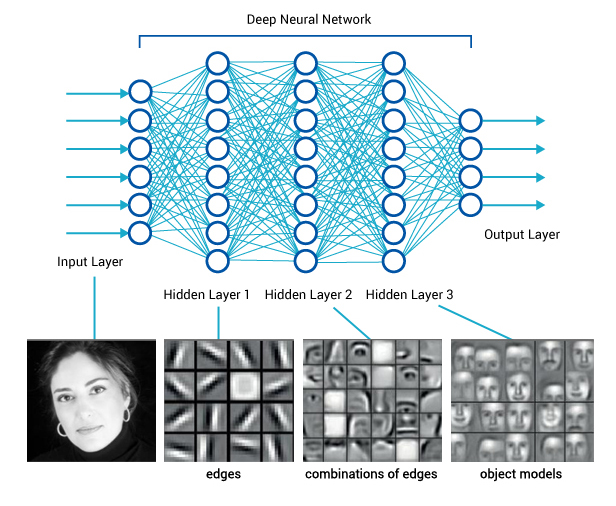
\includegraphics[width=14cm]{blog_deeplearning3.jpg}
					\caption{Illustration of Deep Learning as applied to Vision\label{fig2}}
				\end{figure}	
			\subsection{Convolutional Neural Networks}
			Convolutional Neural Networks (CNN, or ConvNet) are a type of feed-forward artificial neural network in which the connectivity pattern between the neurons is inspired by the organization of the animal visual cortex. Individual cortical neurons respond to stimuli in a restricted region of space known as the \textbf{receptive field}. The receptive fields of different neurons partially overlap such that they tile the visual field. The response of an individual neuron to stimuli within its receptive field can be approximated mathematically by a \textbf{convolution operation}. A Convolutional Neural Network consists of the following layers.
				
			%skipping Relu layer since its not in picture assume it to be in conv layer
				\subsubsection{Convolutional Layer}
					The convolutional layer is the core building block of a CNN. The layer's parameters consist of a set of \textbf{learnable filters} (or kernels), which have a small receptive field, but extend through the full depth of the input volume. During the forward pass, each filter is convolved across the width and height of the input volume, computing the dot product between the entries of the filter and the input and producing a $2$-dimensional activation map of that filter. As a result, the network learns filters that activate when it detects some specific type of feature at some spatial position in the input.

				\subsubsection{Max Pooling Layer}
					It is common to periodically insert a Pooling layer in-between successive Conv layers in a ConvNet architecture. Its function is to \textbf{progressively reduce the spatial size} of the representation to reduce the amount of parameters and computation in the network, and hence to also control overfitting. The Pooling Layer operates independently on every depth slice of the input and resizes it spatially, using the max operation.
				\subsubsection{Fully-Connected Layer}
					Finally, after several convolutional and max pooling layers, the high-level reasoning in the neural network is done via fully connected layers. Neurons in a fully connected layer have \textbf{full connections to all activations} in the previous layer, as seen in regular Neural Networks. Their activations can hence be computed with a matrix multiplication followed by a bias offset. Thus output of the fully connected layer is a vector with elements representing the 'probability' (not in a strictly statistical sense) of the image containing specific objects or actions.
				\begin{figure}[ht!]
					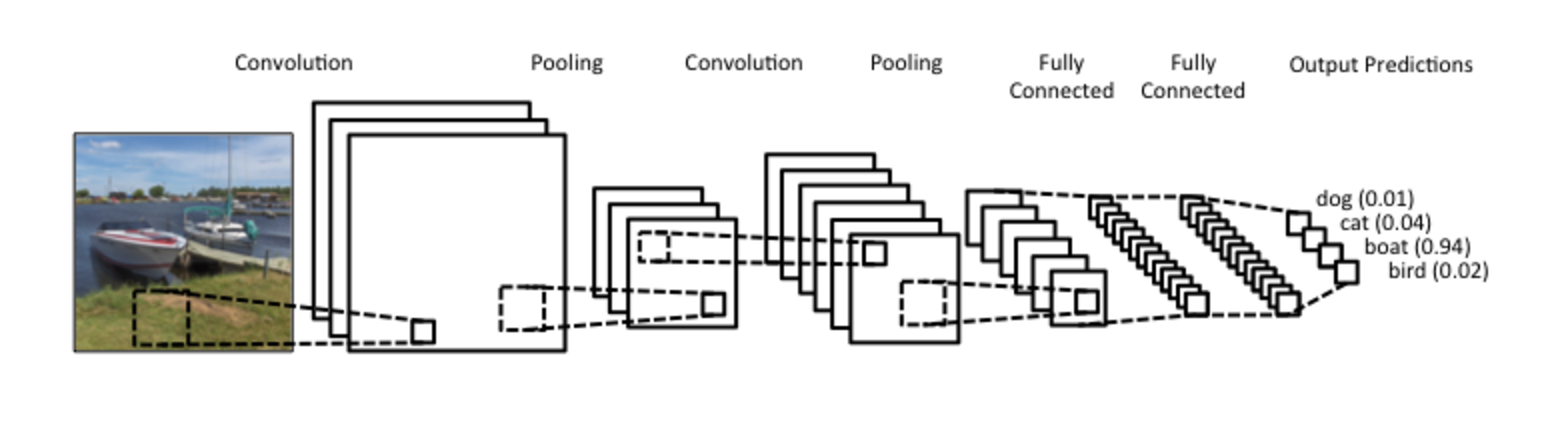
\includegraphics[width=14cm]{conv.png}
					\caption{A Typical Comvolutional Neural Network\label{fig4}}
				\end{figure}
			\subsection{Long Short Term Memory Networks}
			    \begin{figure}[ht!]
					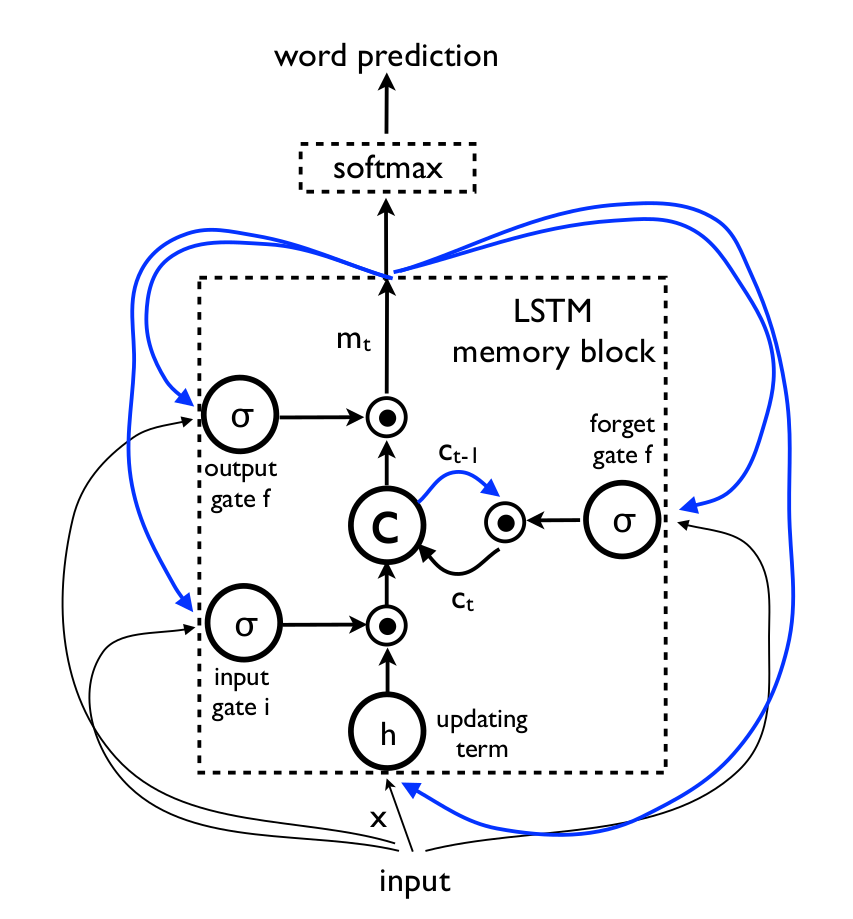
\includegraphics[width=\textwidth]{LSTM_unit.png}
					\caption{A single LSTM unit\label{fig6}}
				\end{figure}
				Long Short Term Memory Networks are a type of Recurrent Neural Networks. Both of them are networks based upon recursion, so that variable length inputs can be handled. LSTM's are specifically used for making RNNs learn long term patterns since traditional RNNs tend to \textbf{favour short term temporal dynamics}. It can be difficult to train traditional RNNs to learn long-term dynamics, likely due in part to the \textbf{vanishing and exploding gradients problem} that can result from propagating the gradients down through the many layers of the recurrent network, each corresponding to a particular time step. LSTMs provide a solution by incorporating memory units that explicitly allow the network to learn when to ``forget'' previous hidden states and when to update hidden states given new information.
				


				
			\subsection{Training Deep Neural Networks}
				A Deep Neural Network is at it's core a parameter based function. All of these parameters are  \textbf{trained} automatically from inputs and expected output tuples (training data). The training process revolves around minimizing a particular cost function using methods like \textbf{Stochastic gradient descent}. The input is given to the network in a feed forward fashion and the parameters aremodified from the last layer to the first (\textbf{Backpropogation}). Neural Networks by design require huge amounts of training data and take a large time to get trained. For some perspective most current state of the art image classifiers have $> 100 million$ parameters and are trained on more than 1.2 million images. 
				\begin{figure}[ht!]
					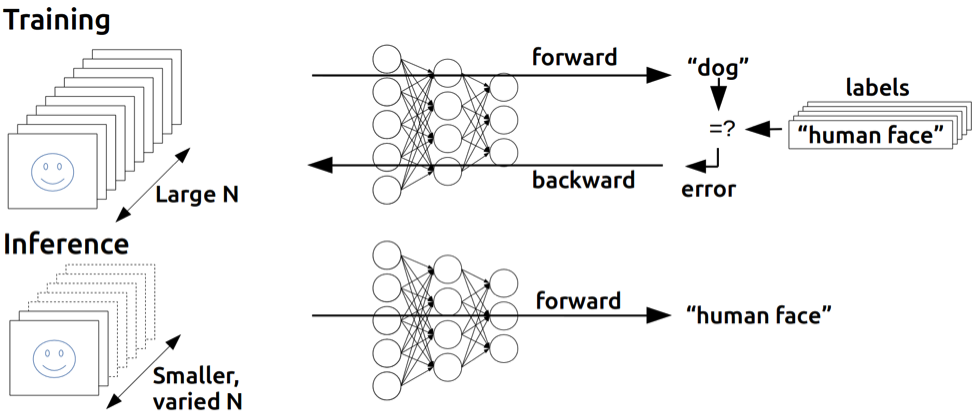
\includegraphics[width=14cm]{training_inference1.png}
					\caption{Training and Inference Processes\label{fig5}}
				\end{figure}

			\subsection{Finetuning}
				Fine-tuning a network is a procedure based on the concept of
				\textbf{transfer learning}. We start training a CNN to learn features for a broad domain with a
				classification function targeted at minimizing error in that domain. Then, we
				replace the classification function and \textbf{optimize the network} again to minimize
				error in another, more specific domain. Under this setting, we are transferring
				the features and the parameters of the network from the broad domain to the
				special one. In our project we will need to use the pre-trained image classification models 
				to actually decode individual frames of the video, thus we are planning to \textbf{fine-tune those models
				with respect to the output of our LSTMs}.




			
		%\end{itemize}


	\section{Approach to the project}
		First, we shall be implementing image captioning in order to be able to encode individual video frames in fixed-length vector represenation of it.
		Then, we will be using our constructed CNN to encode video frames sampled at a fixed interval.
		We will then use RNNs to translate this representation of video into natural language domain. This translation will be achieved by using a set of encoder and decoder RNNs. Since we are working with variable length input and output, we will specifically be using LSTMs for encoding and decoding pursposes as they have been proven to be excellent in machine translation and generalize very well on long data input.
		\begin{enumerate}
			\item Image Captioning
			\begin{enumerate}
				\item
					Construct a VGG/Inception V3 with pre-trained weigths on object classification.
				\item
					Make an LSTM with CNN translated image as input that will be used to translate the image representation into natural language text.
				\item
					Train the model on datasets like MS COCO.
			\end{enumerate}
			\item Video Representation
			\begin{enumerate}
				\item
					We will first sample video at a fixed rate and convert each individual frame to a fixed length vector representation using the CNN trained in image captioning part.
				\item
					We will then try out different approaches of video representation like:
					\begin{itemize}
						\item
							Averaging over all video frame encodings obtained to get a fixed vector representation of video.
						\item
							Using RNNs to encode this variable length video representation.
					\end{itemize}					
			\end{enumerate}
			\item Natural Language Conversion
			\begin{enumerate}
				\item
					Based on how we choose to encode our video, we will have to select appropriate archietecture of LSTM to be used to decode the representation
				\begin{figure}[ht!]
				\centering
					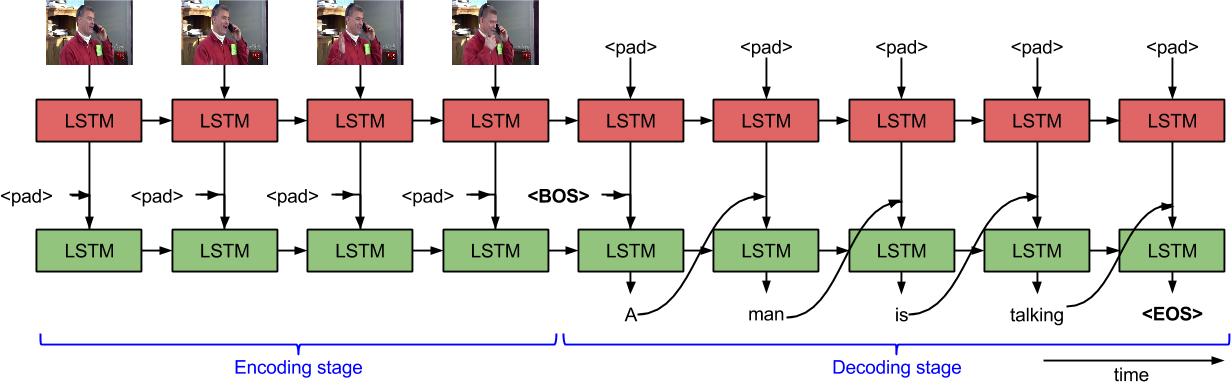
\includegraphics[width=10cm]{s2vt.png}
					\caption{Video description model with 2 LSTM levels\label{fig1}}
				\end{figure}

				\item
					One popular choice(Figure~\ref{fig1}) that we will try out first will be to use a two level LSTM model that will do a sequence to sequence mapping from variable length video representation to variable length natural language sentence.
				\item
					Then we will train our model on the training data we have obtained and plot the learning curves.
				\item
					We will also have to check for over-fitting and under-fitting during our training process and finetune our hyper parameters according to it.
			\end{enumerate}
			\item Further Possibilities
			\begin{enumerate}
				\item We will look for techniques of data augumentation and transfer learning to compensate for the limited amount of training data for video description.
				\item We will also look into some recent techniques of using optical flow for attention modelling which has shown in some cases to improve the results of action recognition.
				\item We will also consider using more efficient vocabulary representation than one hot encoding as vocabulary in this case would be very large.
				\item Try to make forward propagation fast and more memory efficient.
				\item We will also try to develop an end user application that will speak out description of a video that a person shoots.
			\end{enumerate}
		\end{enumerate}

	\section{Datasets}
		Though the source of video description datasets, we have found some viable options that can be worked upon. Even though these are not very large datasets (like MSCOCO) but some research has been done using these and we are confident that we can work using these datasets. Some of them are:
		\begin{enumerate}
		\item
			\textbf{Microsoft Video Description (MSVD)}: The dataset contains 41.2 hours and 200K clip-sentence pairs in total, covering the most comprehensive categories and diverse visual content, and representing the largest dataset in terms of sentence and vocabulary.
		\item
			\textbf{MPII Movie Description Dataset (MPII-MD)}: MPII-MD contains around 68,000 video clips extracted from 94 Hollywood movies. Each clip is accompanied with a single sentence description which is sourced from movie scripts and audio description (AD) data.
		\item
			\textbf{Montreal Video Annotation Dataset (M-VAD)}: The M-VAD movie description corpus is another recent collection of about 49,000 short video clips from 92 movies. It is similar to MPII-MD, but only contains AD data and only provides automatic alignment. 
		\end{enumerate}
%	\section{Approach to the project} 
%		First, we shall be using sensor fusion to obtain accurate estimates for camera position and orientation of the mobile device. Then we will move on to 3D reconstruction, which further has two parts: i.e. sparse 3D reconstruction and then use tracking to obtain dense correspondence of points for dense 3D reconstruction.
%		\begin{enumerate}
%			\item Position and orientation estimation
%			\begin{enumerate}
%				\item
%					Get accelerometer data and orientation data at real time using the IMU sensors like accelerometer, gyroscope, gravity sensor and magnetometer present on the smart phone.
%					This data is highly noisy. Figure~\ref{fig1} shows the position estimate from accelerometer data across various devices.
%
%					\begin{figure}[ht!]
%					\centering
%					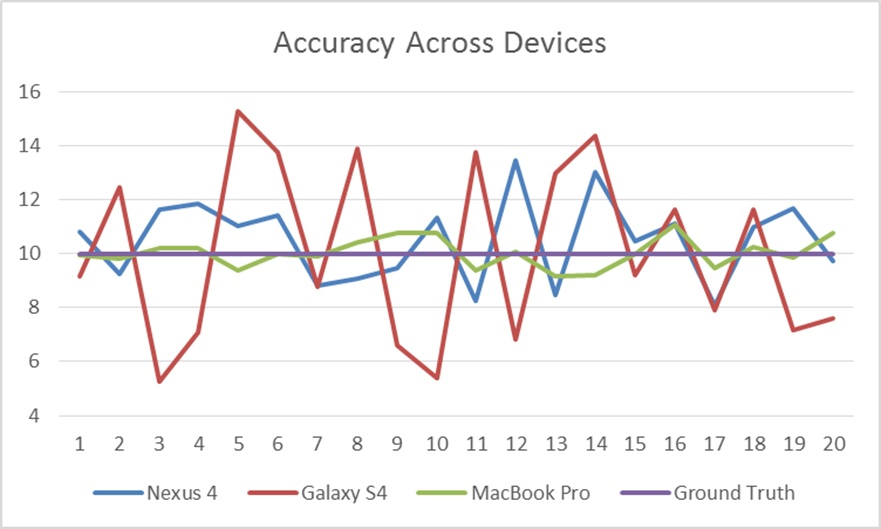
\includegraphics[width=10cm]{graph.jpg}
%					\caption{Accuracy of accelerometer data across different devices (scale cm)\label{fig1}}
%					\end{figure}
%
%					As evident from the graph, this data cannot be directly used for calculation of position and orientation. 
%					Figure~\ref{fig2} shows the integration of static accelerometer data to obtain velocity and displacement.
%
%					\begin{figure}[ht!]
%					\centering
%					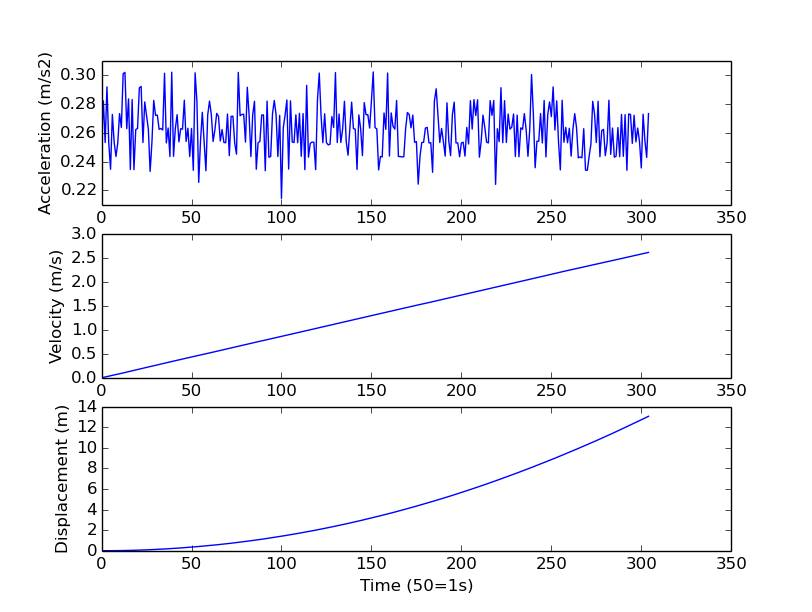
\includegraphics[width=10cm]{integration.jpg}
%					\caption{Obtaining velocity and displacement from static accelerometer data\label{fig2}}
%					\end{figure}
%
%					The graph of both velocity and displacement shows significant deviation from the actual value which is zero.
%					Thus, signal processing and smoothening is required to get a better estimate.
%
%				\item
%					Making the orientation data more accurate by infusing the higher frequency components from the gyroscope orientation after drift correction.
%				\item
%					Obtaining the displacement and orientation data from the camera feed on the device using visual tracking methods.
%				\item
%					A comparative study is to be done between the position estimates obtained by the two methods along with ground truth and fusing the results to obtain an enhanced position and orientation estimate.
%			\end{enumerate}
%			% • All these data along with the clicking of pictures are synchronised to a single system clock.
%			% \item We will use the IMU sensors present in smart-phones to get a position estimation.
%			\item 3D reconstruction
%			\begin{enumerate}
%				\item 
%					Obtain sparse 3D reconstruction based on camera rotation and position parameters obtained previously.
%				\item
%					Use tracking data from different tracking methods like ``Good features to track'' or ``KL tracker'' for obtaining dense correspondence of points.
%				\item
%					Use guided matching by indirect computation of fundamental matrix from estimated camera motion from sensors to further enrich the correspondences.
%				\item
%					Triangulate the dense correspondences and do a final global refinement.					
%			\end{enumerate}
%			\item Further possibilities
%			\begin{itemize}
%			    \item Getting a more detailed texture mapping of the object.
%			    \item Making an object recognition software on the basis of this 3D reconstruction.
%			    \item Improving the algorithm for a quicker and more efficient 3D reconstruction. 
%				\item Releasing applications for Apple, Android and Windows platforms for near real time 3D reconstruction on the device itself.
%			\end{itemize}
%		\end{enumerate}

	
	

	\section{Uses and applications}
	% \item Uses and Applications
			\begin{itemize}
				\item
					Assisting visually impared people to get description of their surrounding, thus enabling them to "see".
				\item
					Very useful for automated survelliance and theft detection but being able to analyze large amounts of data that is not viewable by humans.
				\item
					Allowing content based video retrieval by describing the contents of video in textual format which is indexable by web crawlers.
				\item
					This can also be used to detect catastrophic events through security cameras like fire breakout, murder etc.
				\item
					This project can also be applied in helping robotic vision as this project basically allows one to understand what is happening in the video and thus robots will be able to get a "true" sense of their surroundings.
			\end{itemize}
%			\begin{itemize}
%				\item Using the device as an accurate measuring device. This can be of particular interest to blind as they will be able to measure distances and angles accurately with great ease.
%				\item Doing real time dense 3D reconstructions on mobile phones and other hand-held devices. 
%				\item Allowing the user to generate a 3D printable file on his mobile device. As 3D printers are becoming cheaper and more common, this feature will reduce the need of the person to use a 3D scanner to be able to generate prototypes of objects. This will allow engineers and students to work more efficiently as they can generate copies of 3D objects easily.
%				\item This project can have applications in the field of archeology. It can be used to generate replica of artifacts and fragile objects for further studies, without harming its integrity.
%				\item Our approach can also be applied in the field of medical sciences, especially for orthopedics and joint replacement surgery. The part to be replaced can be made with high accuracy using this project.
%				\item The method can also be used by the astronauts up in space. With the help of our approach the parts to be changed can be easily made using a 3D printer.
%				\item Localization at tourist sites and providing real time directions to landmark locations. This will involve the use of GPS (Global positioning system) as well to get a rough location of the user.
%			\end{itemize}
	\section{Budget and duration}	
		\subsection{Budget}
			No budget is required.
			% Rs. 25,000 will be needed to purchase an android smart phone having high quality sensors and a high resolution camera.
					
		\subsection{Duration}
			We will try to complete this project by the end of the summer break i.e. the end of July, 2017. 
%		\subsection{Facilities}
%		    \begin{itemize}
%		    \item Access to the vision lab.
%		    % \item Access to a computer in Vision Lab.
%		    \end{itemize}
\end{document}
